\documentclass[a4paper,12pt]{ctexart}
% \usepackage{xeCJK}
\usepackage{amsmath}
\usepackage{amsfonts}
\usepackage{float}
\usepackage{enumerate}
\usepackage{graphicx}
\usepackage{tikz}
\usepackage[scale=0.8]{geometry}
\usepackage[hidelinks]{hyperref}
\title{经济学综合第二次作业}
\author{董晨阳 2201211201}
\date{\today}
\begin{document}
\maketitle
\section{黄金法则储蓄率}
\subsection*{a}
稳态时
\begin{equation*}
    \dot k=sy^*-(n+g+\delta)k^*=0
\end{equation*}
即
\begin{equation*}
    y^*=\frac{(n+g+\delta)k^*}{s}
\end{equation*}
从而消费
\begin{equation*}
    c^*=(1-s)y^*= \frac{(1-s)(n+g+\delta)}{s}k^*
\end{equation*}
故
\begin{equation*}
    \frac{\partial c^*}{\partial k^*}=\frac{(1-s)(n+g+\delta)}{s}
\end{equation*}
\subsection*{b}
根据黄金法则
\begin{equation*}
    f'(k^{gold})=n+g+\delta
\end{equation*}
代入$y=k^\alpha$得
\begin{equation*}
    \alpha k^{\alpha-1}=n+g+\delta
\end{equation*}
得到黄金律下
\begin{equation*}
    k^{gold}=\left(\frac{(n+g+\delta)}{\alpha}\right)^{\frac{1}{\alpha-1}}
\end{equation*}
又稳态下有
\begin{equation*}
    k^*=\left(\frac{s}{n+g+\delta}\right)^{\frac{1}{1-\alpha}}
\end{equation*}
解得
\begin{equation*}
    s=\alpha
\end{equation*}
\section{人口与长期产出}
\subsection*{a}\label{sec:a}
平衡增长路径上满足
\begin{equation*}
    sf(k^*)=(n+g+\delta) k^*
\end{equation*}
左右两边对$n$求导得
\begin{equation*}
    sf'(k^*) \frac{\mathrm{d}k^*}{\mathrm{d}n}=k^*+(n+g+\delta)\frac{\mathrm{d}k^*}{\mathrm{d}n}
\end{equation*}
解得
\begin{equation*}
    \frac{\mathrm{d}k^*}{\mathrm{d}n}=\frac{k^*}{sf'(k)-(n+g+\delta)}
\end{equation*}
由于$y^*=f(k^*)$,故
\begin{equation*}
    \frac{\mathrm{d}y^*}{\mathrm{d}n}=\frac{\mathrm{d}y^*}{\mathrm{d}k^*}\cdot\frac{\mathrm{d}k^*}{\mathrm{d}n}=\frac{f'(k^*)k}{sf'(k^*)-(n+g+\delta)}
\end{equation*}
产出弹性为
\begin{equation*}
    \frac{\mathrm{d}y^*}{\mathrm{d}n}\cdot\frac{n}{y^*}=\frac{f'(k^*)k^*n}{(sf'(k^*)-(n+g+\delta))f(k^*)}
\end{equation*}
代入$\alpha_k(k^*)=\displaystyle \frac{k^*f'(k^*)}{f(k^*)}$得
\begin{equation*}
    \frac{\mathrm{d}y^*}{\mathrm{d}n}\cdot\frac{n}{y^*}=\frac{n \alpha_k(k^*)}{sf'(k^*)-(n+g+\delta)}
\end{equation*}
又
\begin{equation*}
    sf'(k^*)=\frac{(n+g+\delta)k^*}{f(k^*)}f'(k^*)=(n+g+\delta)\alpha_k(k^*)
\end{equation*}
故
\begin{equation*}
    \frac{\mathrm{d}y^*}{\mathrm{d}n}\cdot\frac{n}{y^*}=\frac{n}{n+g+\delta}\frac{\alpha_k(k^*)}{\alpha_k(k^*)-1}
\end{equation*}
\subsection*{b}
代入数值计算得
\begin{equation*}
    \frac{\mathrm{d}y^*}{\mathrm{d}n}\cdot\frac{n}{y^*}=-\frac{1}{8}
\end{equation*}
故$n$从2\%下降至1\%的影响估算为导致
\begin{equation*}
    \frac{\Delta y}{y}=-\frac{1}{8}\cdot \frac{\Delta n}{n}=0.0625
\end{equation*}
即$y$增加6.25\%
\section{科技增长减缓与储蓄水平}
\subsection*{a}\label{sec:1}
根据欧拉方程
\begin{equation}
    \frac{\dot c}{c}=\frac{f'(k)-\rho-\theta g}{\theta}=0\label{eq:1}
\end{equation}
科技增长水平下降会导致$f'(k)$减小故$k$增大,因此$\dot c=0$会右移

同理对资本而言,
\begin{equation}
    \dot k=f(k)-c-(n+g)k=0\label{eq:2}
\end{equation}
科技增长水平下降会导致$\displaystyle \dot k>0$,因此$\dot k=0$会上移
\subsection*{b}
从\nameref{sec:1}可知,$k_{NEW}^*>k_{OLD}^*$,此时位于均衡点$E$左侧,因此鞍点路径一定是从左至右的。由于一定存在且只存在一条均衡路径,且只有一个交点,根据相图可知,鞍点路径来自于左下向右上直至新均衡点。又由于$\dot k$右移过,因此在$k_{old}$处消费新的$\dot k=0$更低,如图\ref{fig:1}所示,因而瞬间点消费一定会更小,因而会减小
\begin{figure}[H]
    \centering
    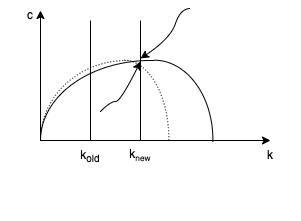
\includegraphics[trim=0 60 0 0,width=0.5\linewidth]{fig/fuck.drawio.png}
    \caption{示意图}\label{fig:1}
\end{figure}
\subsection*{c}
根据(\ref{eq:1})(\ref{eq:2})可知平衡增长路径上
\begin{eqnarray}
    f'(k)&=&\rho+\theta g \label{eq:4}\\
    f(k)&=&c+(n+g)k\label{eq:5}
\end{eqnarray}
故$$s=\frac{k(n+g)}{f(k)}$$
从而
\begin{eqnarray}
    \frac{\partial s}{\partial g}&=&\frac{(k+(n+g)\frac{\partial k}{\partial g})f(k)-f'(k)k(n+g)\frac{\partial k}{\partial g}}{(f(k))^2}\nonumber\\
    &=&\frac{kf(k)+(n+g)(f(k)-f'(k)k)\frac{\partial k}{\partial g}}{(f(k))^2}\label{eq:3}
\end{eqnarray}
分项看:
\begin{enumerate}
    \item $kf(k)>0$显然成立
    \item 由于$f'(k)>0,f''(k)<0$,求导可知$f(k)-f'(k)k$递增,故$f(k)-f'(k)k>f(0)=0$
    \item $\frac{\partial k}{\partial g}$根据\nameref{sec:a}可知是大于0的
\end{enumerate}
综上$\frac{\partial s}{\partial g}>0$恒成立
\subsection*{d}
将$f(k)=k^\alpha$代入(\ref{eq:3})得
\begin{equation}\label{eq:final}
    \frac{\partial s}{\partial g}=\frac{k+(n+g)(1-\alpha)\frac{\partial k}{\partial g}}{k^\alpha}
\end{equation}
结合(\ref{eq:4})有
\begin{equation*}
    \frac{\partial{k}}{\partial{g}}=\frac{\theta}{\alpha(\alpha-1)k^{\alpha-2}}
\end{equation*}
代入(\ref{eq:final})解得
\begin{equation}
    \frac{\partial s}{\partial g}=\frac{\alpha}{\rho+\theta g}\left(1-\frac{\theta(n+g)}{\rho+\theta g}\right)
\end{equation}
\end{document}
